\documentclass{standalone}
\usepackage{tikz}
\usetikzlibrary{patterns}
\usetikzlibrary{positioning}
\usetikzlibrary{patterns, positioning}
\usetikzlibrary{shapes.misc}
\usepackage[outline]{contour}
\contourlength{1.5pt} 
\usepackage[sfdefault]{ClearSans}

\begin{document}
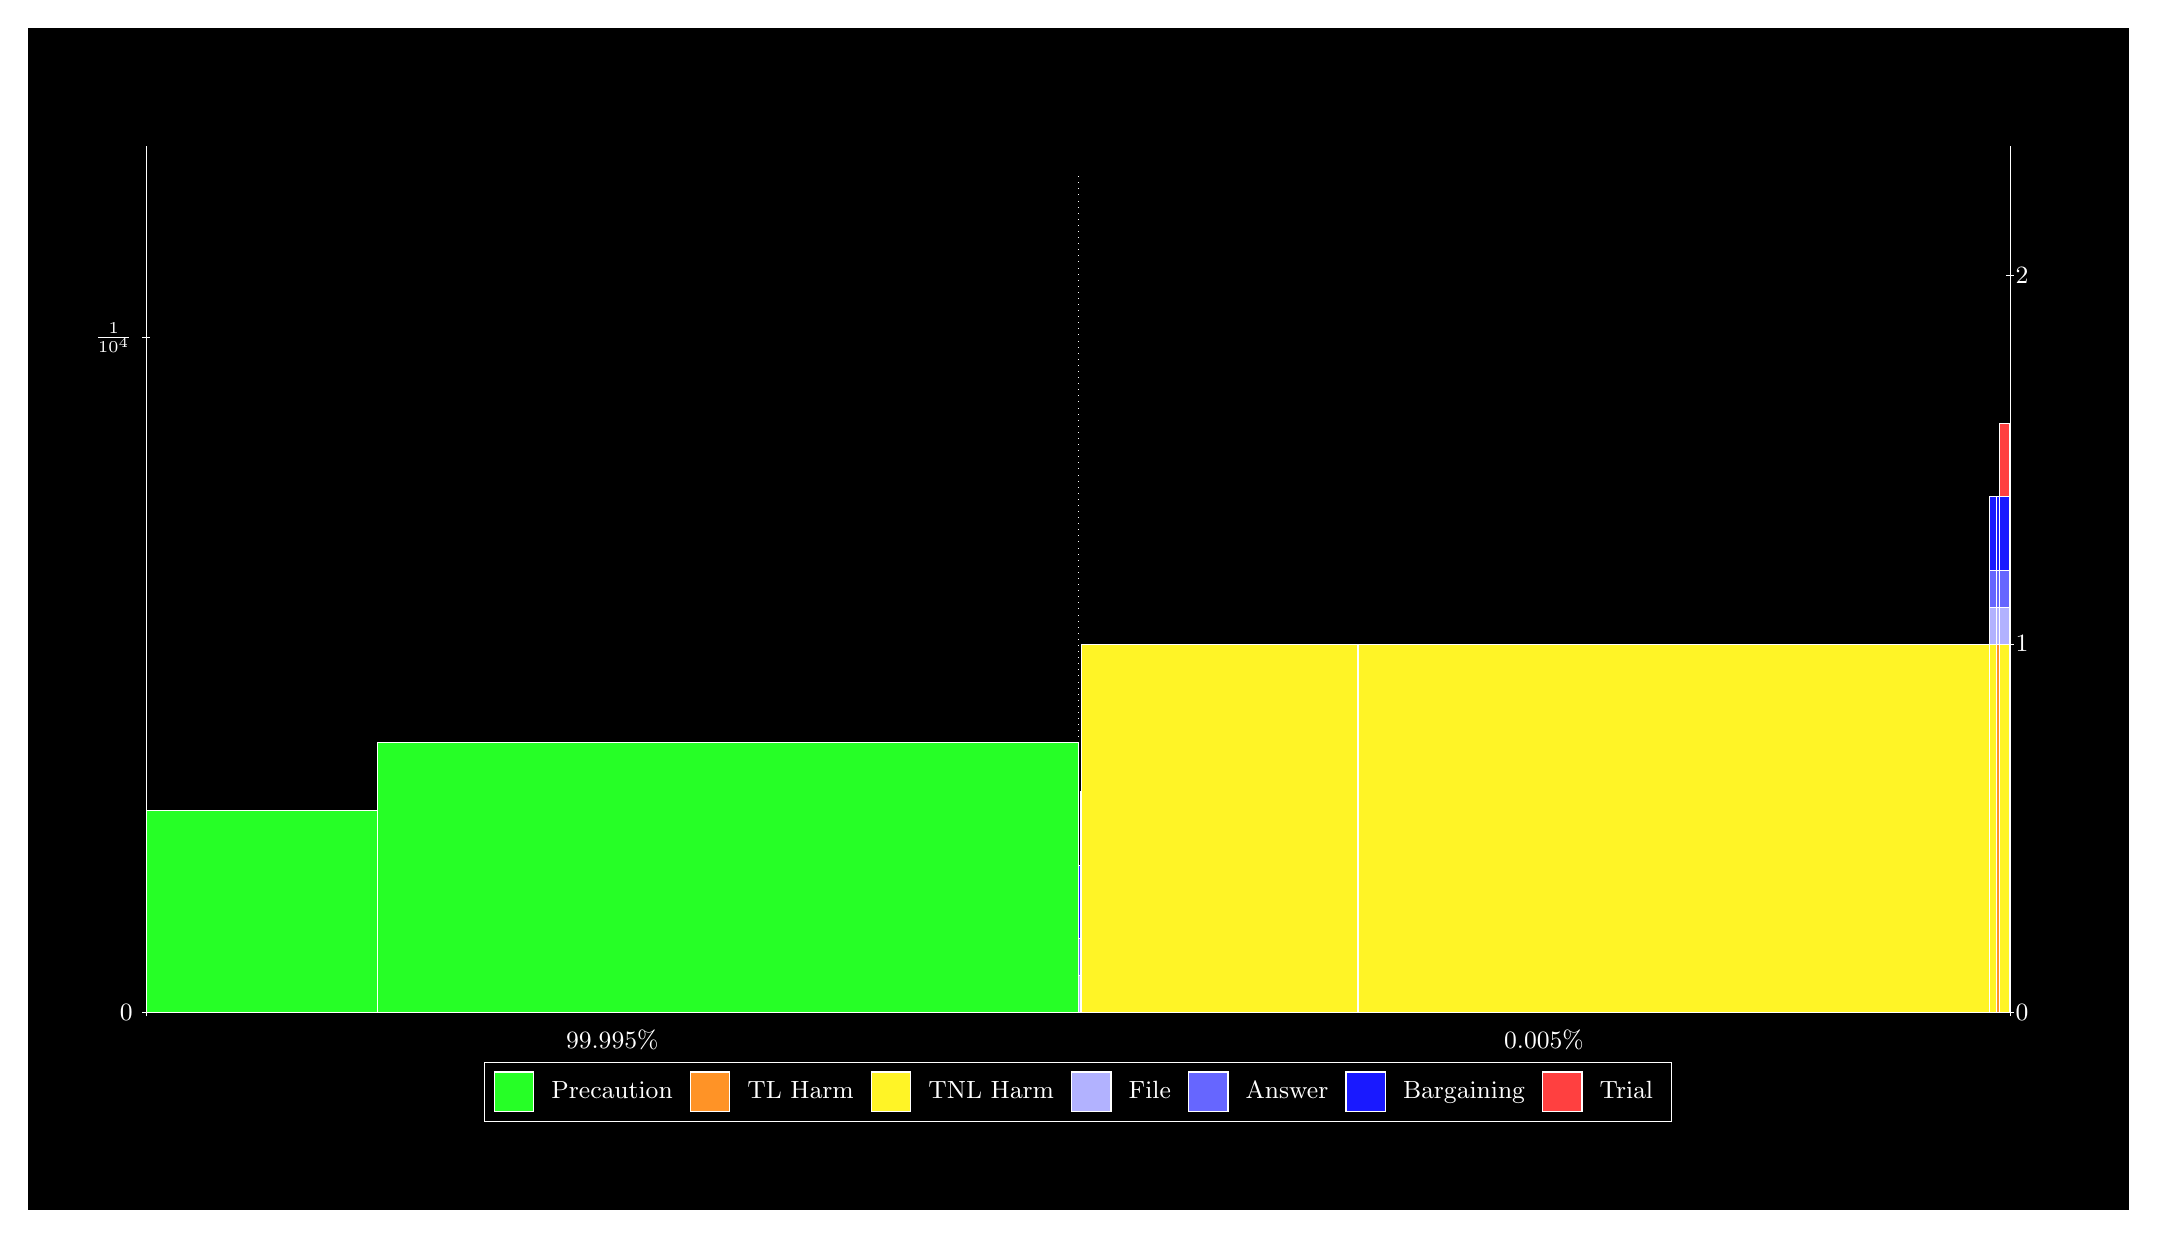
\begin{tikzpicture}
\draw[fill=black] (0,0) rectangle (26.667,15);
\draw[fill=green!85,draw=white,very thin] (1.5,2.5) rectangle (4.4357,5.0715);
\draw[fill=green!85,draw=white,very thin] (4.4357,2.5) rectangle (13.333,5.9287);
\draw[fill=green!85,draw=white,very thin] (13.333,2.5) rectangle (13.356,2.5001);
\draw[fill=blue!30,draw=white,very thin] (13.333,2.5001) rectangle (13.356,2.9682);
\draw[fill=blue!60,draw=white,very thin] (13.333,2.9682) rectangle (13.356,3.4362);
\draw[fill=blue!90,draw=white,very thin] (13.333,3.4362) rectangle (13.356,4.3723);
\draw[fill=green!85,draw=white,very thin] (13.356,2.5) rectangle (13.377,2.5001);
\draw[fill=blue!30,draw=white,very thin] (13.356,2.5001) rectangle (13.377,2.9682);
\draw[fill=blue!60,draw=white,very thin] (13.356,2.9682) rectangle (13.377,3.4362);
\draw[fill=blue!90,draw=white,very thin] (13.356,3.4362) rectangle (13.377,4.3723);
\draw[fill=red!75,draw=white,very thin] (13.356,4.3723) rectangle (13.377,5.3084);
\draw[fill=green!85,draw=white,very thin] (13.377,2.5) rectangle (16.875,2.5001);
\draw[fill=yellow!85,draw=white,very thin] (13.377,2.5001) rectangle (16.875,7.1806);
\draw[fill=green!85,draw=white,very thin] (16.875,2.5) rectangle (16.897,2.5001);
\draw[fill=orange!85,draw=white,very thin] (16.875,2.5001) rectangle (16.897,7.1806);
\draw[fill=green!85,draw=white,very thin] (16.897,2.5) rectangle (24.902,2.5002);
\draw[fill=yellow!85,draw=white,very thin] (16.897,2.5002) rectangle (24.902,7.1807);
\draw[fill=green!85,draw=white,very thin] (24.902,2.5) rectangle (24.994,2.5001);
\draw[fill=yellow!85,draw=white,very thin] (24.902,2.5001) rectangle (24.994,7.1806);
\draw[fill=blue!30,draw=white,very thin] (24.902,7.1806) rectangle (24.994,7.6487);
\draw[fill=blue!60,draw=white,very thin] (24.902,7.6487) rectangle (24.994,8.1167);
\draw[fill=blue!90,draw=white,very thin] (24.902,8.1167) rectangle (24.994,9.0528);
\draw[fill=green!85,draw=white,very thin] (24.994,2.5) rectangle (25.037,2.5001);
\draw[fill=orange!85,draw=white,very thin] (24.994,2.5001) rectangle (25.037,7.1806);
\draw[fill=blue!30,draw=white,very thin] (24.994,7.1806) rectangle (25.037,7.6487);
\draw[fill=blue!60,draw=white,very thin] (24.994,7.6487) rectangle (25.037,8.1167);
\draw[fill=blue!90,draw=white,very thin] (24.994,8.1167) rectangle (25.037,9.0528);
\draw[fill=green!85,draw=white,very thin] (25.037,2.5) rectangle (25.156,2.5001);
\draw[fill=yellow!85,draw=white,very thin] (25.037,2.5001) rectangle (25.156,7.1806);
\draw[fill=blue!30,draw=white,very thin] (25.037,7.1806) rectangle (25.156,7.6487);
\draw[fill=blue!60,draw=white,very thin] (25.037,7.6487) rectangle (25.156,8.1167);
\draw[fill=blue!90,draw=white,very thin] (25.037,8.1167) rectangle (25.156,9.0528);
\draw[fill=red!75,draw=white,very thin] (25.037,9.0528) rectangle (25.156,9.9889);
\draw[fill=green!85,draw=white,very thin] (25.156,2.5) rectangle (25.167,2.5001);
\draw[fill=orange!85,draw=white,very thin] (25.156,2.5001) rectangle (25.167,7.1806);
\draw[fill=blue!30,draw=white,very thin] (25.156,7.1806) rectangle (25.167,7.6487);
\draw[fill=blue!60,draw=white,very thin] (25.156,7.6487) rectangle (25.167,8.1167);
\draw[fill=blue!90,draw=white,very thin] (25.156,8.1167) rectangle (25.167,9.0528);
\draw[fill=red!75,draw=white,very thin] (25.156,9.0528) rectangle (25.167,9.9889);
\draw[white,very thin] (1.5,2.5) -- (1.5,13.5);
\draw[white,very thin] (1.45,2.5) -- (1.55,2.5);
\node[font=\small,text=white, anchor=east] at (1.45, 2.5) {0};
\draw[white,very thin] (1.45,11.072) -- (1.55,11.072);
\node[font=\small,text=white, anchor=east] at (1.45, 11.072) {$\frac{1}{10^{4}}$};

\draw[white,dotted,very thin] (13.333,2.83) -- (13.333,13.17);
\draw[white,very thin] (25.167,2.5) -- (25.167,13.5);
\draw[white,very thin] (25.117,2.5) -- (25.217,2.5);
\node[font=\small,text=white, anchor=west] at (25.117, 2.5) {0};
\draw[white,very thin] (25.117,7.1805) -- (25.217,7.1805);
\node[font=\small,text=white, anchor=west] at (25.117, 7.1805) {1};
\draw[white,very thin] (25.117,11.861) -- (25.217,11.861);
\node[font=\small,text=white, anchor=west] at (25.117, 11.861) {2};

\draw[white,very thin] (1.5,2.5) -- (25.167,2.5);
\draw[white,very thin] (1.5,2.45) -- (1.5,2.55);
\node[font=\small,text=white, anchor=north] at (1.5, 2.45) {};
\draw[white,very thin] (25.167,2.45) -- (25.167,2.55);
\node[font=\small,text=white, anchor=north] at (25.167, 2.45) {};

\node[font=\small,text=white,anchor=south] at (7.4167, 1.9) {99.995\%};
\node[font=\small,text=white,anchor=south] at (19.25, 1.9) {0.005\%};
\draw (13.3333,2.5) node (B) {};
\begin{scope}[align=center]
\matrix[scale=0.5,draw=white,below=0.5cm of B,nodes={draw},column sep=0.1cm]{
\node[rectangle,draw,minimum width=0.5cm,minimum height=0.5cm,fill=green!85]{}; & \node[draw=none,font=\small,text=white]{Precaution}; &
\node[rectangle,draw,minimum width=0.5cm,minimum height=0.5cm,fill=orange!85]{}; & \node[draw=none,font=\small,text=white]{TL Harm}; &
\node[rectangle,draw,minimum width=0.5cm,minimum height=0.5cm,fill=yellow!85]{}; & \node[draw=none,font=\small,text=white]{TNL Harm}; &
\node[rectangle,draw,minimum width=0.5cm,minimum height=0.5cm,fill=blue!30]{}; & \node[draw=none,font=\small,text=white]{File}; &
\node[rectangle,draw,minimum width=0.5cm,minimum height=0.5cm,fill=blue!60]{}; & \node[draw=none,font=\small,text=white]{Answer}; &
\node[rectangle,draw,minimum width=0.5cm,minimum height=0.5cm,fill=blue!90]{}; & \node[draw=none,font=\small,text=white]{Bargaining}; &
\node[rectangle,draw,minimum width=0.5cm,minimum height=0.5cm,fill=red!75]{}; & \node[draw=none,font=\small,text=white]{Trial}; \\\\
};\end{scope}

\end{tikzpicture}
\end{document}